\documentclass{beamer}

\usetheme{Berkeley}
\title{An efficient sampling algorithm for plotting}
\author{Angus Griffith}
\date{January 7, 2015}

\newtheorem*{ex}{Example}
% \usepackage{algorithm,algorithmic}
\usepackage{algpseudocode}

\begin{document}
\begin{frame}
\titlepage
\end{frame}

\section{Motivation}
\begin{frame}
\frametitle{When might function evaluation be slow?}
\begin{itemize}
\item
Searching parameter space for complex scientific calculations (weather modeling, computational chemistry, etc.).
\item
Complex analytic expressions coming from Computer Algebra Systems (Mathematica, Sage, etc.).
\item
Plotting functions which require non-standard evaluation (e.g. integrals, sums).
\item
Limited computational power (e.g. graphics calculators, phones.)
\end{itemize}
\end{frame}

\begin{frame}
\frametitle{Example: Error function}
\[
erf(x) := \frac{2}{\sqrt{\pi}} \int_0^x e^{-t^2} dt,
\]
\begin{figure}
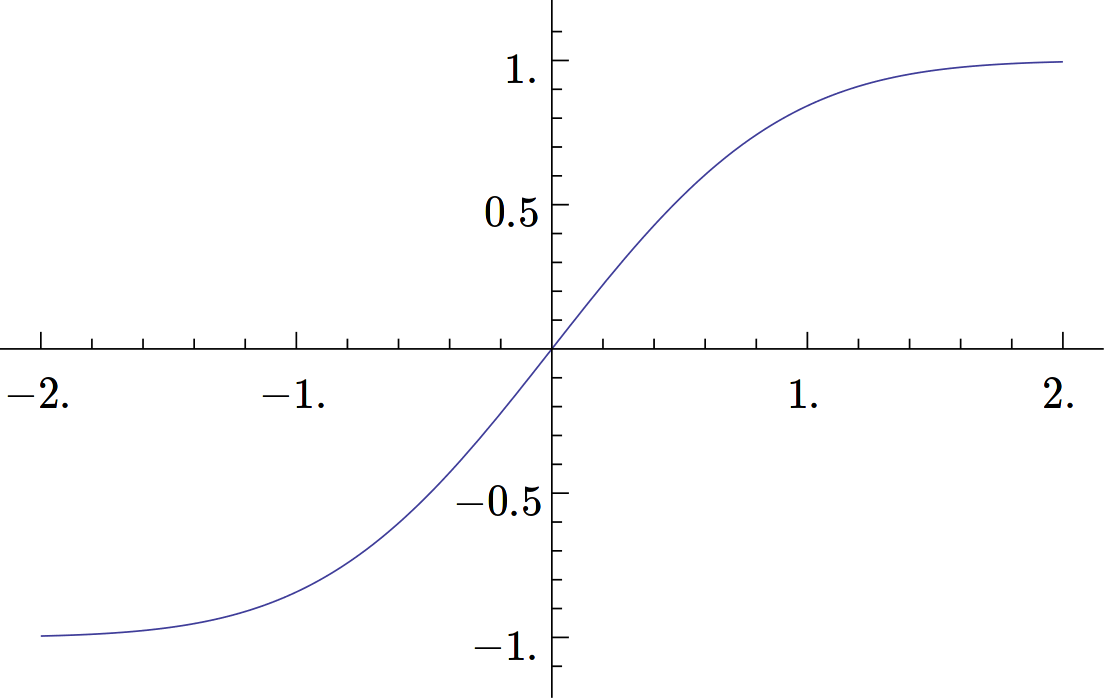
\includegraphics[width=0.5\textwidth]{erfx.png}
\caption{$erf(x)$ for $x \in [-2, 2]$.}
\end{figure}
This function does not have an elementary expression.
\end{frame}

\section{Formalism}
\begin{frame}
\frametitle{Plotting in 2D}
Consider the function $f : [a,b] \subset \mathbb{R} \to \mathbb{R}^2$.
Given a strictly monotone finite sequence $(t_i)_{i=0}^n \subset [a,b]$ we define a plot of $f$ to be the sequence of lines$\big(\left(f(t_{i-1}), f(t_{i})\right)\big)_{i=1}^n.$
\\ \vspace{0.2cm}
{\bf Example:}
To plot the $\sin$ function we pick $f(t) := (t, \sin(t))$. \\ \vspace{0.2cm}
{\bf Example:}
To plot a circle pick $a = 0$, $b = 2\pi$, and $f(t) := (\sin(t), \cos(t))$. \\
\centering
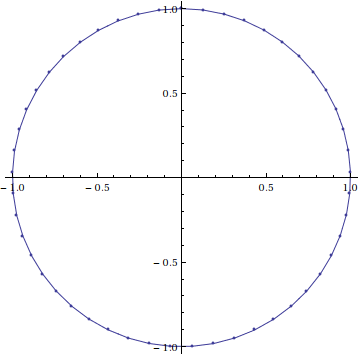
\includegraphics[width=0.4\textwidth]{circle.png}
\end{frame}

\begin{frame}
\frametitle{Plotting in 3D}
We have two possible types of plot: \\ \vspace{0.2cm}
{\bf Lines:}
The same as plotting in 2D (except the lines lie in $\mathbb{R}^3$). \\ \vspace{0.2cm}
{\bf Surfaces:}
Let $D \subset \mathbb{R}^2$ be connected and consider the function $f : D \to \mathbb{R}^3$.
Given a finite sequence $(t_i)_{i=0}^n$ a plot of $f$ is a \emph{triangulation} of the evaluation points $\big(f(t_i)\big)_{i=1}^n$. \\ \vspace{0.2cm}
{\bf Example:}
To plot a sphere, $D = [-\pi, \pi] \times [-\pi, \pi]$ and $f = (\sin(u) \sin(v), \cos(u) \sin(v), \cos(v))$. \\
\centering
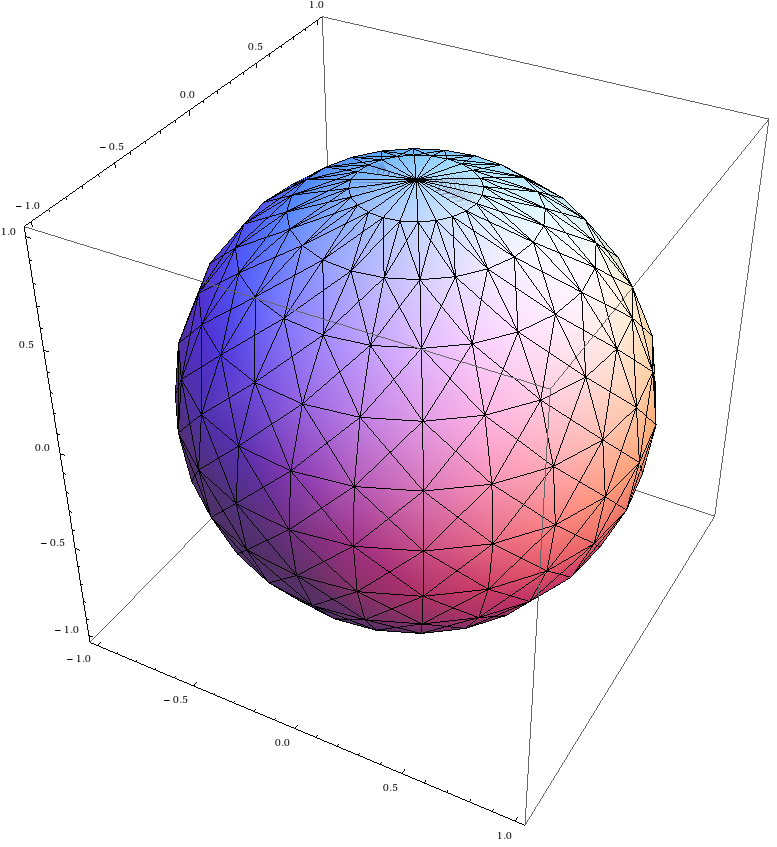
\includegraphics[width=0.3\textwidth]{sphere.png} \\
\end{frame}

\section{Sampling}
\subsection{2D}
\begin{frame}
\frametitle{Linear Sampling}
In order to plot a function $f$ we need to choose a grid of points at which we evaluate $f$. \\ \vspace{0.2cm}
The simplest sampling approach is {\bf linear sampling}. \vspace{0.5cm}
\footnotesize
\begin{algorithmic}[1]
\Function{sample}{$f$, $n$, $a$, $b$}
\State $points \gets []$
\For{$i \gets 0$ to $n$}
\State $t \gets a + i * (b-a) / n$
\State \Call{append}{$points$, $(t, f(t))$}
% \State $points[i] \gets f(t)$
\EndFor
\State \Return $points$
\EndFunction
\end{algorithmic}%  \\ \vspace{0.5cm}
\normalsize
\end{frame}

% \begin{frame}
% \frametitle{A false start: derivative sampling}
% Idea: \\
% Make the density of points proportional to the curvature? \\ \vspace{0.3cm}
% Computing the derivates of $f$ may be difficult (or impossible!).
% \\ \vspace{0.5cm}
% A possible approach: \\
% Linear sampling $\to$ finite differences $\to$ resampling. \\
% An indirect method.
% \end{frame}

\begin{frame}
\begin{center}
  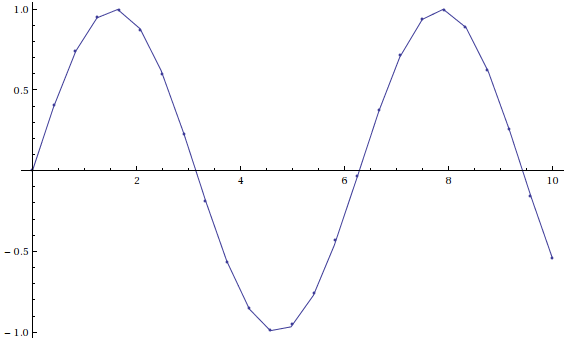
\includegraphics[width=0.7\textwidth]{sinlinear.png} \\
  $n = 25$, $f(t) = (t, \sin(t))$, $[a,b] = [0,10]$. \\ \vspace{0.2cm}
\end{center}
Why does the plot look rough?  \\ \vspace{0.2cm}
We notice the angles between subsequent lines.
\end{frame}

\frametitle{Angle based adaptive resampling}
\begin{frame}
\footnotesize
\begin{algorithmic}[1]
\Function{resample}{$f$, $points$, $\theta$}
\State $newpoints \gets []$
\For{$i \gets 1$ to \Call{len}{$points$}-1}
\State $t_0, p_0 \gets points[i-1]$
\State $t_1, p_1 \gets points[i]$
\State $t_2, p_2 \gets points[i+1]$
\State $s_0 \gets 0.5*(t_0 + t_1)$
\State $s_1 \gets 0.5*(t_1 + t_2)$
\If{\Call{angle}{$p_1 - p_0$, $p_2 - p_1$} $> \theta$}
\State \Call{append}{$newpoints$, $(s_0, f(s_0))$}
\State \Call{append}{$newpoints$, $(s_1, f(s_1))$}
\ElsIf{$i = 1$}
\State \Call{append}{$newpoints$, $(s_0, f(s_0))$}
\ElsIf{$i = $\Call{len}{$points$}-1}
\State \Call{append}{$newpoints$, $(s_1, f(s_1))$}
\EndIf
\EndFor
\State \Return \Call{merge}{$points$, $newpoints$}
\EndFunction
\end{algorithmic}
\normalsize
\end{frame}

\begin{frame}
We repeat resampling until all no offending angles remain or we hit a recursion limit
\footnotesize
\begin{algorithmic}[1]
\State $points \gets$ \Call{sample}{$f$, $n$, $a$, $b$}
\For{$depth \gets 1$ to $max\_depth$}
\State $points \gets $\Call{resample}{$f$, $points$, $\theta$}
\EndFor
\end{algorithmic} \vspace{-0.3cm}
\pause
\begin{center}
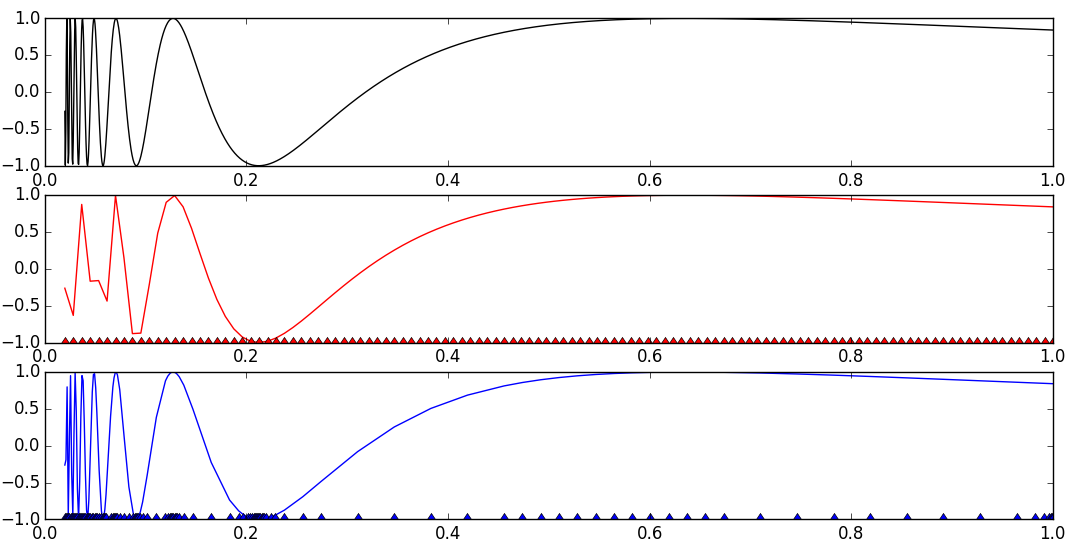
\includegraphics[width=0.8\textwidth]{comparison.png} \\
\end{center}
$f(t) = (t, sin(1/t))$, $[a,b] = [0.02, 1]$, $n = 25$, $max\_depth = 5$, $\theta = \pi / 10$.
\normalsize
\end{frame}

\begin{frame}
Zooming in on the region $[0.02, 0.2] \times [-1,1]$
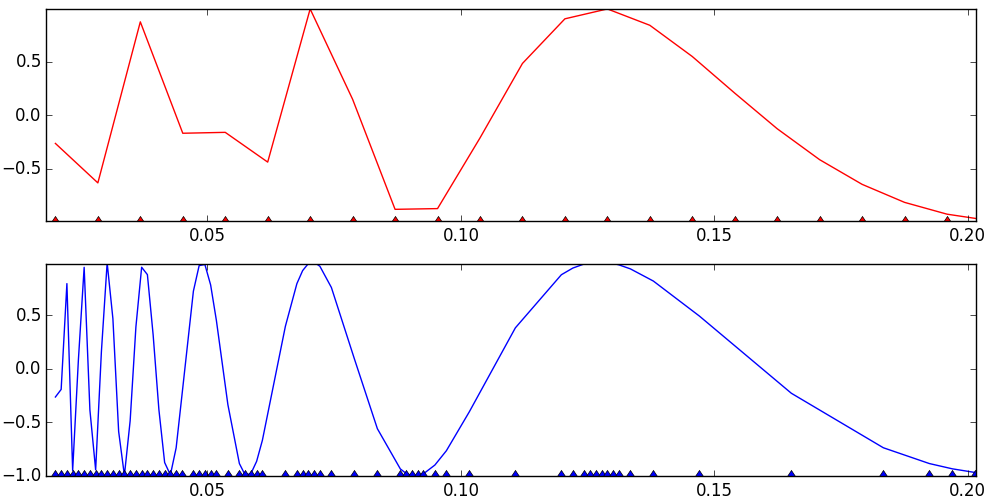
\includegraphics[width=\textwidth]{comparison_zoom.png} \\
\footnotesize
$f(t) = (t, sin(1/t))$, $[a,b] = [0.02, 1]$, $n = 27$, $max\_depth = 5$, $\theta = \pi / 18$.
\normalsize
\end{frame}

\begin{frame}
\frametitle{However}
\footnotesize
Knowing the algorithm it is easy to pick a function which will plot badly. \\
\begin{center}
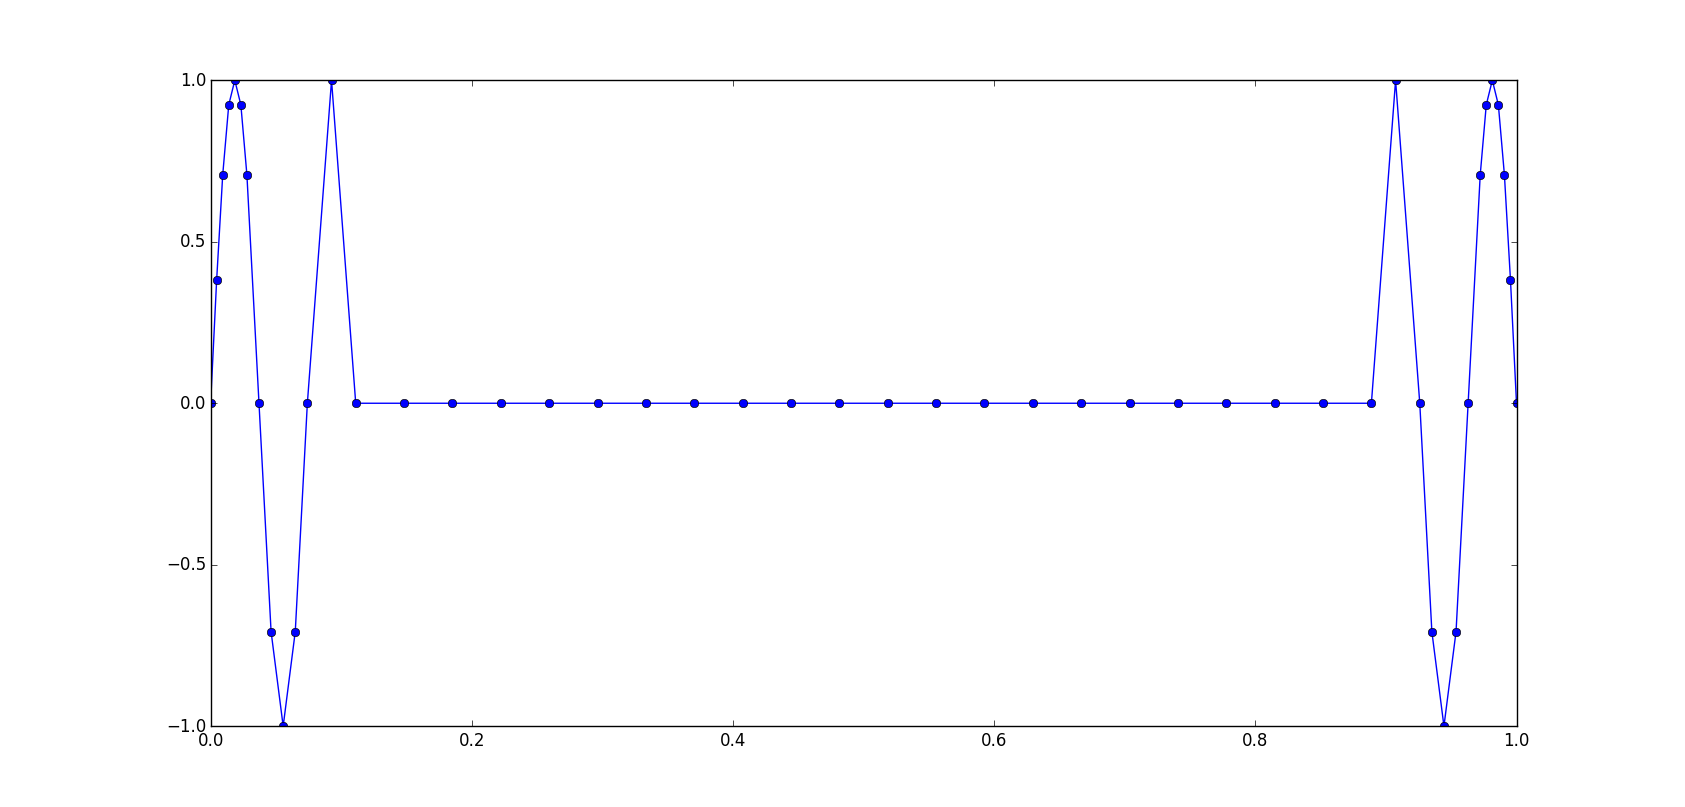
\includegraphics[width=\textwidth]{evil.png}
\end{center}
$[a,b] = [0, 1]$, $n = 27$, $max\_depth = 5$, $\theta = \pi / 18$,
\pause
$f(t) = (t, \sin(27 \pi t))$.
\normalsize
\end{frame}

\subsection{3D}
\begin{frame}
\frametitle{Linear sampling}
\begin{center}
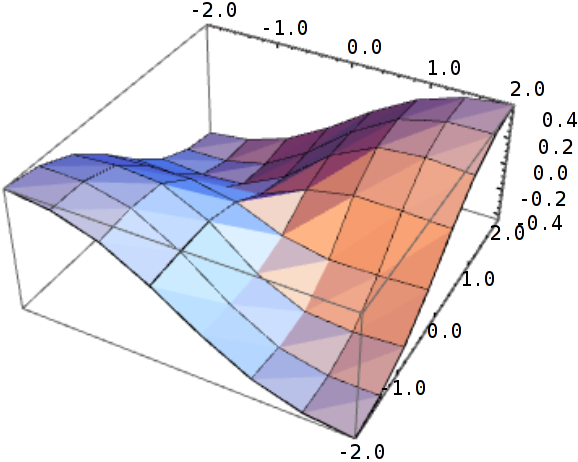
\includegraphics[width=0.8\textwidth]{3Dsimple.png}
\end{center}
$f(x,y) = \left(x,y, \frac{x y}{x^2 + y^2 + 1}\right)$, $n = 7$.
\end{frame}

\begin{frame}
\frametitle{Linear sampling minimising diagonals}
\begin{center}
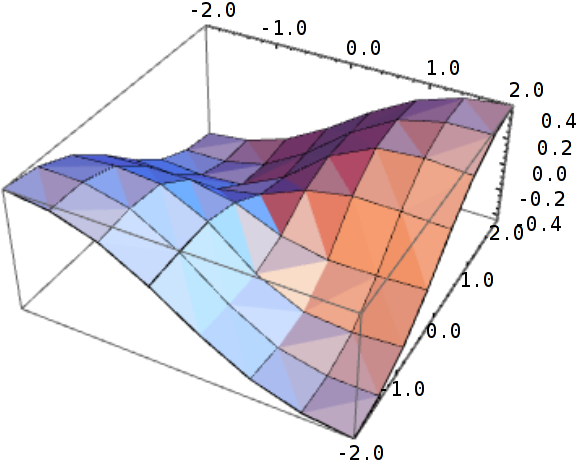
\includegraphics[width=0.8\textwidth]{3Dlinear.png}
\end{center}
$f(x,y) = \left(x,y, \frac{x y}{x^2 + y^2 + 1}\right)$, $n = 7$.
\end{frame}

\begin{frame}
\frametitle{Adaptive sampling minimising diagonals}
\begin{center}
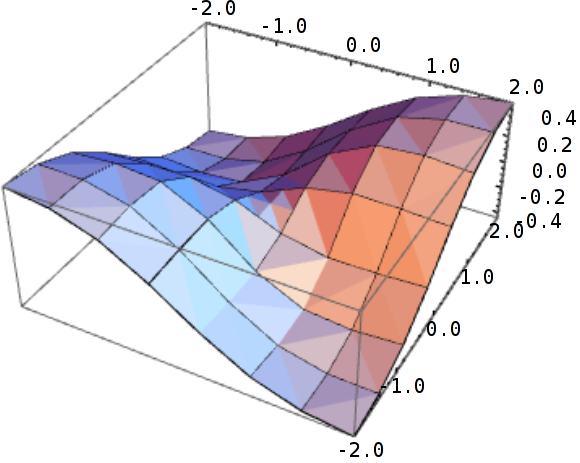
\includegraphics[width=0.8\textwidth]{3Dadaptive.png}
\end{center}
$f(x,y) = \left(x,y, \frac{x y}{x^2 + y^2 + 1}\right)$, $n = 7$, $depth=2$.
\end{frame}

\section*{}
\begin{frame}
\frametitle{Thankyou}
\url{https://github.com/sn6uv/adaptive_plotting/}

\end{frame}

\end{document}
